\section{Evaluation}

\subsection{Methodology}

The evaluation answers five questions:

\begin{enumerate}[leftmargin=*]
\item Does \system avoid relying on an easy PQC-only trace?
\item Does \system remove stale-secret exposure on DOGI-style workload axes?
\item Under pressure, does \system reduce WAF and GC relative to history-based placement?
\item What overhead does semantic placement introduce?
\item What security claim is supported by actual device capability?
\end{enumerate}

\noindent\textbf{Evaluation platform.}
We evaluate placement with trace-driven replay and an actual \zns device: a Western Digital ZN540-class NVMe SSD exposed as \texttt{/dev/nvme0n1} and mounted through \texttt{zonefs}.  The replay model uses 4KiB logical blocks and a 275,712-block zone capacity.  As in DOGI's methodology, the simulator/replay path gives broad policy coverage, while the physical path validates that the planned append/reset schedule executes on a zoned device.  Because the full-suite path includes zonefs helper overhead, we report its latency as overhead accounting rather than production SPDK p99 latency.

\noindent\textbf{Baselines.}
We compare against FIFO, \sepbit-style, \midas-style, and \dogi-style placement.  These are same-path policies in our simulator and actual-\zns replay.  We also keep exact public DOGI/MiDAS/SepBIT runs as separate evidence because their internal units are not directly interchangeable with our packed \zns replay.

\noindent\textbf{Workloads.}
The fairness matrix uses six DOGI-style axes: FIO Zipf, YCSB-A, YCSB-F, Varmail, Alibaba, and Exchange.  Headline WAF rows keep these locality signals and add PQC lifecycle side writes through high-ratio YCSB-A/F, FAST-style Sysbench-OLTP pressure, and dynamic Exchange/Varmail/Alibaba-like traces.  Pure PQC epoch streams are sanity checks, not headline evidence.  Hostile robustness uses tenant mixing, missing hints, wrong hints, and stragglers; real FIO iolog and Sysbench/MySQL gates check benchmark readiness.

\noindent\textbf{Metrics.}
We report WAF, GC write blocks, stale secret blocks, semantic physical reset count, secret bytes waiting for physical reset, zone utilization, live physical zones, append/reset latency, and C-level placement-decision overhead.  A stale secret block is an expired secret-class logical block in a family that is not safely reset- or sanitize-eligible because live data remains or epoch close is unproven.  Exposure artifacts report stale-secret block-seconds; physical tables use final and representative stale-block counts for auditability.  WAF alone is insufficient because a policy can keep WAF near 1.0 while leaving expired PQC secrets in mixed zones.
For example, the E4 exposure timeline records max stale-secret block-seconds of 69,391,500 for FIFO and \dogi-style placement, while \system remains at zero block-seconds and zero final stale-secret blocks.

\subsection{Workload Hardness}

The workload hardness rule is: DOGI-friendly first, PQC-hostile second.  A headline WAF/GC row must preserve storage-visible structure that helps history-based placement---hot/cold skew, overwrite locality, segment reuse, or phase changes---and then add PQC objects whose invalidation follows protocol state rather than LBA history.  Pure PQC-only traces, oracle-expiration traces, and low-pressure rows are sanity checks or exposure evidence.

The matrix passes all nine gates: fairness, negative controls, pressure rows, main-claim eligibility, and hostile robustness.  The artifact set has seven eligible YCSB pressure rows, nine YCSB baseline-complete rows, three dynamic eligible rows, and DB pressure eligibility.  Rows with WAF near 1.0 are interpreted as semantic exposure results; WAF/GC claims come only from rows where history-based policies pay positive GC or copied-live-block cost.

\subsection{Epoch Upper Bound}

DOGI uses NoDaP as an oracle-like target for lost lifetime information.  We use a narrower upper bound: an epoch oracle that sees exact death time at write time.  It is not deployable and is not counted as \system; it tests whether the workload is placeable once the protocol-lifetime signal exists.

On the mixed sanity trace, \dogi-style placement has WAF 1.791 and 484,967 GC blocks, \system has WAF 1.010 and 6,331 GC blocks, and the epoch oracle has WAF 1.000 and zero GC blocks.  On the stress-rekey trace, \dogi-style placement has WAF 2.031, \system has WAF 1.019, and the oracle has WAF 1.003.  These synthetic rows are bounds, not headline evidence: most of the gap comes from whether the allocator can observe the protocol lifetime boundary.

\begin{figure*}[t]
\centering
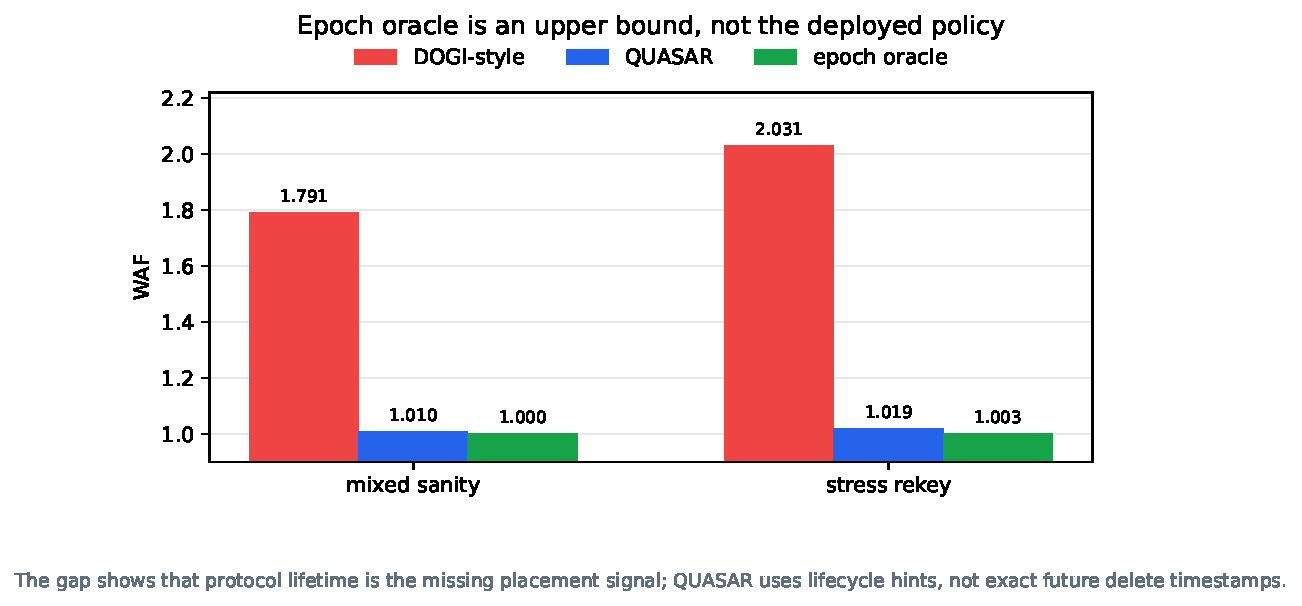
\includegraphics[width=0.72\textwidth]{../artifacts/figures/paper/epoch-upper-bound.pdf}
\caption{Epoch upper bound.  The epoch oracle is not a deployable baseline; it receives exact future death time.  Its role is to show that the WAF gap is largely a missing-lifetime-signal problem.  \system approaches the upper bound with lifecycle hints, while the paper's headline claims still come from harder physical-\zns pressure rows.}
\label{fig:epoch-upper-bound}
\end{figure*}

\subsection{DOGI-Favorable Control}

The non-PQC control verifies that the hybrid preserves history placement.  On the six DOGI-style axes with no PQC side writes, \dogi-style placement and the \system-\dogi hybrid produce the same WAF because payload stays on the history policy.  \dogi-style placement beats FIFO and pure \system on all six workloads, and no stale secret blocks exist.  This keeps the claim boundary clear: \system is not a replacement for learned placement when no cryptographic death-cohort signal exists.

\subsection{Same-Path Fairness Matrix}

The six-axis actual-\zns fairness matrix completes 72 rows with zero failures.  Table~\ref{tab:fairness} reports the aggregated policy results.  \dogi-style placement is already strong on WAF, which is expected on an easy fairness matrix.  However, it leaves 99,834 stale secret blocks and performs no semantic physical resets.  \system-\dogi hybrid leaves zero stale secret blocks, performs 98 semantic resets, and reduces GC blocks from 625 to 106.

\begin{table}[t]
\centering
\caption{Same-path actual-\zns fairness matrix over six DOGI-style axes at pqc2000.  The easy matrix keeps \dogi-style WAF near 1.0, but only \system-\dogi hybrid removes stale secrets while reducing GC.}
\label{tab:fairness}
\footnotesize
\begin{tabularx}{\columnwidth}{lRRRR}
\toprule
\textbf{Policy} & \textbf{WAF} & \textbf{GC} & \textbf{Stale secrets} & \textbf{Resets} \\
\midrule
FIFO & 1.0040 & 3,903 & 99,141 & 0 \\
\sepbit-style & 1.0023 & 2,241 & 99,822 & 0 \\
\midas-style & 1.0006 & 581 & 99,898 & 0 \\
\dogi-style & 1.0006 & 625 & 99,834 & 0 \\
\system & 1.0011 & 1,121 & 0 & 98 \\
\system-\dogi hybrid & 1.0001 & 106 & 0 & 98 \\
\bottomrule
\end{tabularx}
\end{table}

The WAF gain here is deliberately modest: 0.1\% relative to \dogi-style.  The row is a semantic result, not a performance headline: storage-history placement can have good WAF and still fail to make expired PQC secrets resettable.

\subsection{YCSB Pressure}

YCSB pressure creates the WAF/GC separation missing from easy p2000 rows.  Table~\ref{tab:ycsb} reports representative physical \zns replays.  \dogi-style placement pays 3,357--24,289 GC blocks and leaves 46,266--150,221 stale secret blocks.  The hybrid removes stale secret blocks in all rows and reduces GC to zero in these representative replays.

\begin{table*}[t]
\centering
\caption{Representative actual-\zns YCSB pressure replays.  These traces keep YCSB update locality while adding PQC lifecycle side writes, showing where pressure turns the semantic gap into measurable GC/WAF cost.}
\label{tab:ycsb}
\footnotesize
\begin{tabularx}{\textwidth}{lRRRRRRR}
\toprule
\textbf{Workload} & \textbf{DOGI WAF} & \textbf{Hybrid WAF} & \textbf{DOGI GC} & \textbf{Hybrid GC} & \textbf{DOGI stale} & \textbf{Hybrid stale} & \textbf{Hybrid resets} \\
\midrule
YCSB-A pqc4000 & 1.0454 & 1.0000 & 15,316 & 0 & 46,266 & 0 & 28 \\
YCSB-A pqc6000 & 1.0376 & 1.0000 & 15,308 & 0 & 76,950 & 0 & 28 \\
YCSB-A pqc10000 & 1.0066 & 1.0000 & 3,357 & 0 & 150,221 & 0 & 26 \\
YCSB-F pqc6000 & 1.0105 & 1.0000 & 4,166 & 0 & 96,050 & 0 & 28 \\
YCSB-F pqc8000 & 1.0528 & 1.0000 & 24,289 & 0 & 100,847 & 0 & 28 \\
YCSB-F pqc10000 & 1.0279 & 1.0000 & 13,741 & 0 & 144,901 & 0 & 26 \\
\bottomrule
\end{tabularx}
\end{table*}

The p10000 rows bound the WAF claim.  Dense YCSB overlays can keep \dogi-style WAF close to 1.0, yet the stale-secret gap remains large.  WAF improvement appears under pressure; exposure improvement appears across PQC overlays.

\subsection{Multi-Seed Ratio Sweep}

To check that the pressure result is not a single-seed artifact, we run a three-seed ratio sweep over the six DOGI-style workload families at 0\%, 5\%, and 20\% PQC overlay ratios, for 54 comparisons.  The hybrid matches \dogi-style at 0\% PQC, is WAF-negative at 5\% PQC (-1.1\% mean WAF, -12.4\% mean GC) while avoiding 2,342 stale secret blocks per seed, and becomes positive at 20\% PQC (5.0\% mean WAF and 38.3\% mean GC improvement) while avoiding 10,021 stale secret blocks per seed.  Thus low-ratio overlays are exposure evidence, not WAF wins; WAF/GC benefits appear once protocol-lifetime objects create enough placement pressure.

\subsection{DB and Dynamic-Service Pressure}

Table~\ref{tab:pressure} reports the harder Sysbench and dynamic service rows.  Sysbench is not a DOGI-paper workload; it is included as FAST-style DB pressure.  The hybrid reduces \dogi-style GC from 11,256 to 609 blocks and removes 38,438 stale secret blocks.  On Exchange-, Varmail-, and Alibaba-like dynamic traces, the hybrid reduces GC by 92.3--99.9\% and keeps stale secrets at zero.

\begin{figure*}[t]
\centering
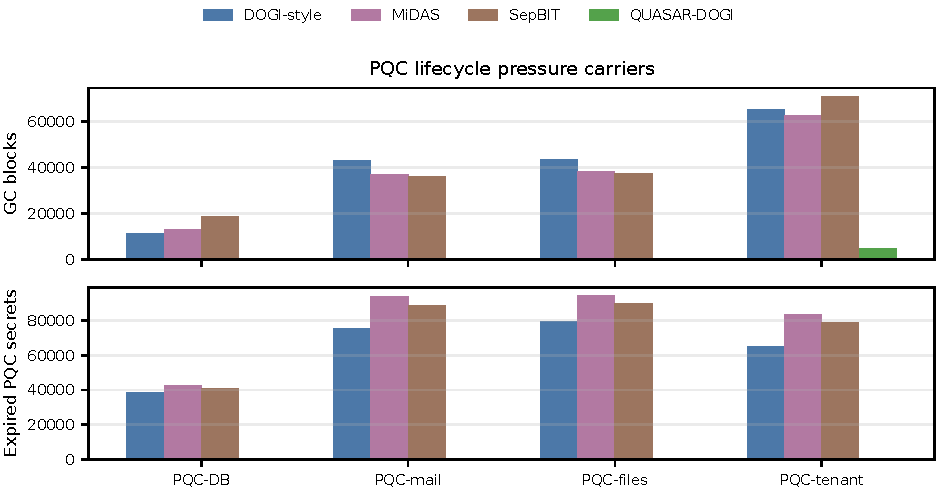
\includegraphics[width=0.88\textwidth]{../artifacts/figures/fast-style/fig2-pressure-breadth.pdf}
\caption{FAST-style pressure breadth.  Sysbench, Exchange, Varmail, and Alibaba-like rows keep storage-visible locality while adding PQC lifecycle objects.  History-based policies can still group payload, but they do not make expired secret cohorts reset-eligible; \system-\dogi cuts GC and stale-secret exposure on the same pressure axes.}
\label{fig:pressure-breadth}
\end{figure*}

\begin{table*}[t]
\centering
\caption{FAST-style DB and dynamic-service pressure.  Dynamic rows use DOGI-style workload families with high PQC overlays and tight logical-zone pressure; the hybrid preserves zero stale secrets while cutting GC.}
\label{tab:pressure}
\footnotesize
\begin{tabularx}{\textwidth}{lRRRRRRR}
\toprule
\textbf{Workload} & \textbf{DOGI WAF} & \textbf{Hybrid WAF} & \textbf{DOGI GC} & \textbf{Hybrid GC} & \textbf{DOGI stale} & \textbf{Hybrid stale} & \textbf{GC reduction} \\
\midrule
Sysbench-OLTP pressure & 1.0301 & 1.0016 & 11,256 & 609 & 38,438 & 0 & 94.6\% \\
Exchange-like pqc8000 & 1.0716 & 1.0000 & 43,006 & 22 & 75,422 & 0 & 99.9\% \\
Varmail-like pqc8000 & 1.0727 & 1.0003 & 43,227 & 175 & 79,600 & 0 & 99.6\% \\
Alibaba-like pqc8000 & 1.0974 & 1.0075 & 65,010 & 4,992 & 65,184 & 0 & 92.3\% \\
\bottomrule
\end{tabularx}
\end{table*}

These rows are the strongest performance evidence because all non-QUASAR baselines complete but pay visible GC and leave stale secrets.  They also show why the hybrid is the default deployable policy: payload placement remains history-based, while secrets are placed by protocol cohort.

\subsection{Component Ablation}

Table~\ref{tab:ablation} turns the upper-bound requirements into mechanism evidence.  History-only placement is the right first row because it gives \dogi-style placement all storage-visible signals but no protocol lifetime.  Adding lifecycle hints removes stale secrets, but pure semantic grouping can still leave GC cost on DB-like payload.  Adding the \dogi payload fallback removes that remaining cost.  Admission and residual migration are not free performance wins; they are boundary mechanisms for open-zone pressure and stragglers.  Figure~\ref{fig:component-ablation} shows the mechanism split visually, and Figure~\ref{fig:resource-overhead} visualizes the space and overhead controls.

\begin{figure*}[t]
\centering
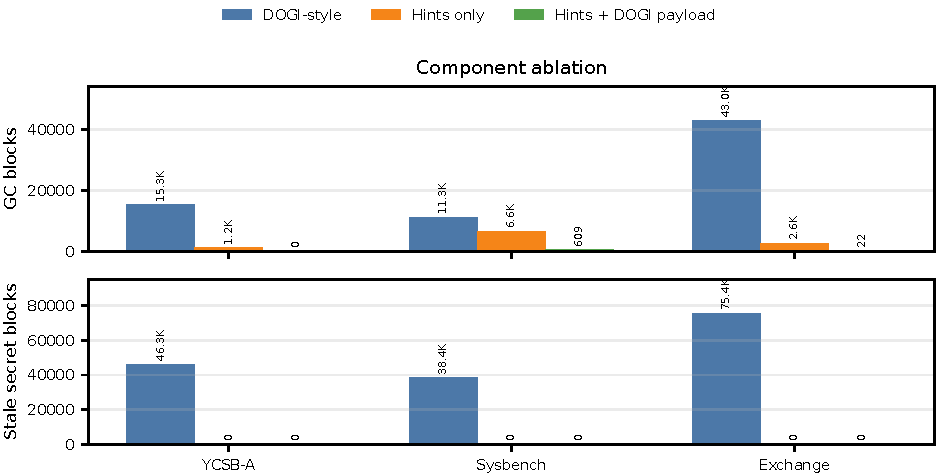
\includegraphics[width=0.88\textwidth]{../artifacts/figures/fast-style/fig3-component-ablation.pdf}
\caption{Component ablation.  A history-only \dogi-style policy sees storage history but misses death cohorts, so GC and stale-secret exposure remain.  Lifecycle hints remove exposure; adding \dogi-style payload fallback recovers payload placement and removes the remaining GC in the default hybrid.}
\label{fig:component-ablation}
\end{figure*}

\begin{table*}[t]
\centering
\caption{Component ablation from actual-\zns and pressure artifacts.  Lifecycle hints remove stale secrets, the \dogi payload fallback recovers payload GC behavior, and residual migration exposes the cost of strict zero-wait security.}
\label{tab:ablation}
\scriptsize
\begin{tabularx}{\textwidth}{lYYY}
\toprule
\textbf{Component} & \textbf{Evidence} & \textbf{Lesson} & \textbf{Decision} \\
\midrule
History only & DOGI YCSB-A p4000: GC 15,316, stale 46,266, resets 0. & History misses protocol death. & Do not place secrets by history alone. \\
Lifecycle hints & Pure \system: YCSB-A stale 0; Exchange stale 0. & Hints carry the missing signal. & Route PQC objects by death cohort. \\
Payload fallback & Hybrid cuts Sysbench GC 6,567$\rightarrow$609 and Exchange GC 2,610$\rightarrow$22. & Payload still needs history. & Keep \dogi fallback as default. \\
Admission & Exact hybrid wins 6 YCSB/Sysbench rows; adaptive wins 0. & Binning is not free. & Use adaptive only under pressure. \\
Residual & Stragglers: binning caps 13 zones but leaves 40,454 waiting; residual reaches 0 at WAF 1.7098. & Strict exposure has copy cost. & Expose low/strict profiles. \\
\bottomrule
\end{tabularx}
\end{table*}

\subsection{Exact Public Baseline Sanity Runs}

The main tables use same-path replay so FIFO, \sepbit-style, \midas-style, \dogi-style, \system, and the hybrid share trace timing, packed physical-\zns model, and reset accounting.  We also ran public baseline artifacts in their native environments.  Public DOGI completes Alibaba p8000 compact, selector-suite, and original-LBA runs with reported WAF 2.993, 2.804, and 3.212; public MiDAS completes compact FIO and PQC representatives with WA 1.000 and 1.250; public SepBIT completes a PQC pressure representative with WA 2.430.  These runs are sanity evidence, not apples-to-apples WAF numbers.  They sharpen the boundary: MiDAS is strong on at least one compact representative, so the claim rests on death-cohort exposure and same-path pressure evidence, not universal baseline collapse.

\subsection{Overhead}

\system adds semantic reset work, but its decision path is cheap.  In the actual-\zns overhead suite, the hybrid issues 318 more semantic reset operations than \dogi-style.  Zonefs-helper throughput is lower than \dogi-style by this accounting, but helper latency includes user-space append/truncate overhead.  In the C-level placement-decision benchmark, \dogi-style feature extraction plus a small MLP costs 2,397.8 ns/write, \system hint routing costs 16.8 ns/write, and the hybrid costs 1,178.8 ns/write.

The xNVMe probe provides a lower-overhead command-path sanity check: 4,096 4KiB zone appends complete with p99 latency of 26,064 ns and throughput of 181.79 MiB/s.  The probe is a Linux NVMe ioctl path, not SPDK poll-mode, so it is reported as a bound rather than a final production datapoint.

\begin{figure*}[t]
\centering
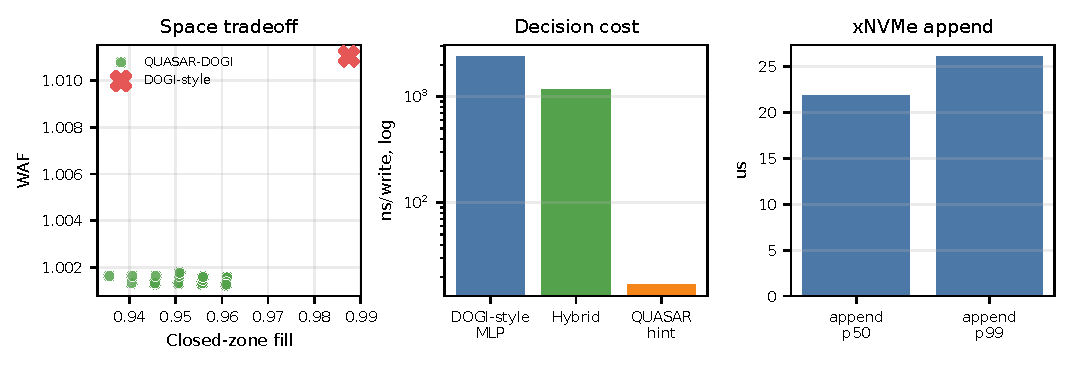
\includegraphics[width=0.88\textwidth]{../artifacts/figures/fast-style/fig4-resource-overhead.pdf}
\caption{Resource and overhead controls.  \system-\dogi bounds the closed-zone fill cost while removing stale secrets, the hint-routing decision path is orders of magnitude cheaper than the \dogi-style policy-decision microbenchmark, and xNVMe confirms a lower-overhead append command path than the zonefs helper used for full-suite replay accounting.}
\label{fig:resource-overhead}
\end{figure*}

\subsection{Robustness to Bad Hints and Stragglers}

The hardest \system cases are not clean epochs; they are wrong or missing hints, many tenants, and delayed-expiry stragglers.  On YCSB-A p4000, the clean hybrid has WAF 1.0000, zero stale secrets, and 28 semantic resets.  With 5\% missing hints, WAF remains 1.0000 but 3,361 stale secret blocks appear because some secret writes fall back to nonsemantic placement.  With 5\% wrong epochs, this trace still ends with zero stale secrets but increases reset activity to 112 resets.  With 5\% stragglers, exact secret-group packing can exceed the device open-zone budget; epoch-bin fallback completes within the budget but leaves waiting secrets, while epoch-bin plus residual migration reaches zero waiting at WAF 1.7098 after copying 234,549 residual blocks.

The residual fallback frontier shows why strict exposure mode cannot be the default.  Exchange-like and Sysbench-like representatives can reach zero final secret waiting with physical WAF 1.0182 and 1.2161, respectively.  YCSB-F p8000 reaches strict zero waiting only at physical WAF 3.5535 after migrating 1,168,095 residual blocks.  \system therefore exposes low-overhead, balanced, and strict-zero-wait profiles rather than hiding this tradeoff behind a single policy.

\begin{figure*}[t]
\centering
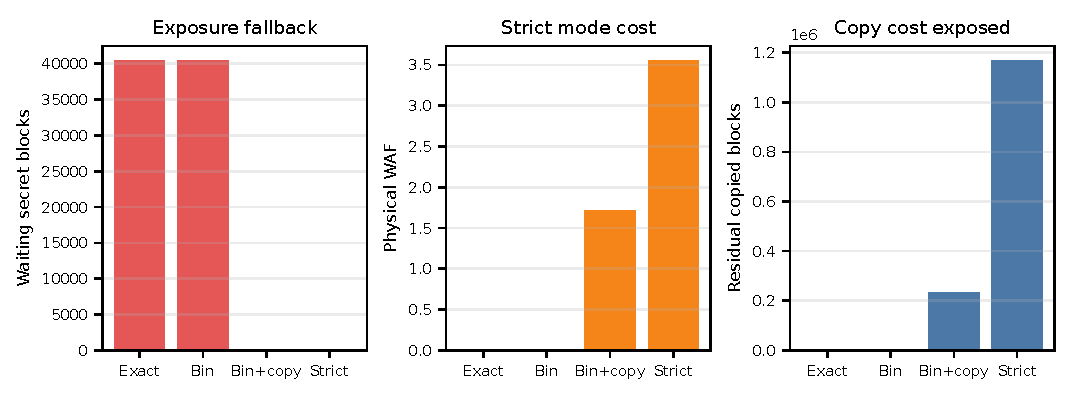
\includegraphics[width=0.88\textwidth]{../artifacts/figures/fast-style/fig6-robustness.pdf}
\caption{Robustness frontier.  Exact and binned placement can leave straggler secrets waiting under tight active-zone budgets.  Residual migration removes the exposure but increases physical WAF and copied blocks; strict zero-wait mode is therefore a policy point, not the default.}
\label{fig:robustness}
\end{figure*}

\subsection{Security Boundary}

The physical device advertises crypto-erase and block-erase sanitize support.  We executed crypto-erase sanitize and observed successful completion in the sanitize log.  This supports a deployment path where \system triggers hardware erase semantics at epoch boundaries.  The default result remains more conservative: \system reduces stale-secret exposure by aligning secret lifetime with reset eligibility, while physical erasure requires explicit sanitize or equivalent hardware support.  We do not use sanitize timing to claim foreground service latency: sanitize policy, batching, and SLO integration are deployment choices beyond the same-path placement comparison.

\subsection{Reproducibility}

The artifact manifest records 37 evidence artifacts, their roles, abbreviated hashes, and regeneration commands.  Validation finds zero hash mismatches, and the local acceptance report passes 41 of 41 gates.  These checks make the scoped evidence auditable.
